\documentclass[tikz, border=16pt]{standalone}
\usepackage{tikz}
\usetikzlibrary{shapes.geometric, arrows.meta, positioning, fit, backgrounds}

\begin{document}
\begin{tikzpicture}

  %% Left: Python diagram
  \node[inner sep=0pt, anchor=north west] (left) at (0,0) {%
    \begin{tikzpicture}[node distance=0.7cm]
      \input{control_flow_python_content}
    \end{tikzpicture}%
  };

  %% Right: R diagram — top-aligned, offset 1cm to the right
  \node[inner sep=0pt, anchor=north west] (right) at ([xshift=1cm]left.north east) {%
    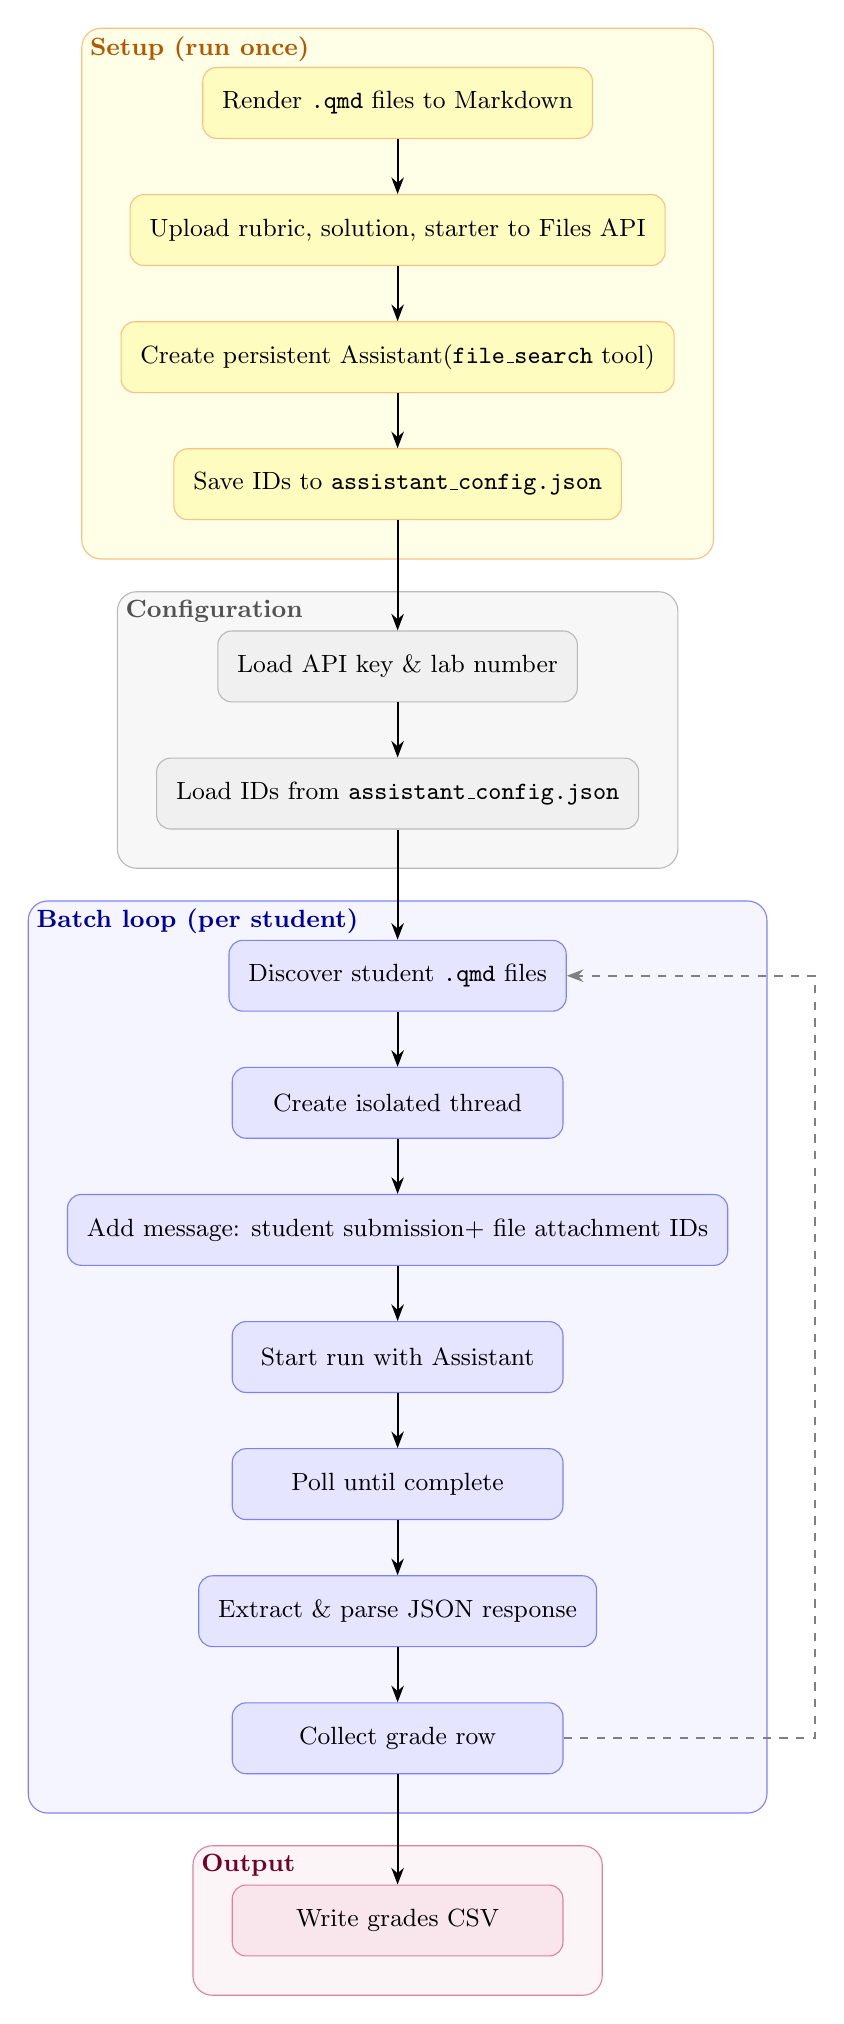
\begin{tikzpicture}[node distance=0.7cm]
      \tikzset{
  box/.style={
    rectangle, rounded corners=5pt, draw, text centered,
    minimum width=4.2cm, minimum height=0.9cm,
    font=\small, inner sep=7pt
  },
  arrow/.style={-{Stealth[length=6pt]}, thick},
  darrow/.style={-{Stealth[length=6pt]}, thick, dashed, gray},
  config/.style  ={box, fill=gray!12,   draw=gray!55},
  setup/.style   ={box, fill=yellow!25, draw=orange!50},
  core/.style    ={box, fill=blue!10,   draw=blue!50},
  outnode/.style ={box, fill=purple!10, draw=purple!50},
  grouplabel/.style={font=\small\bfseries, anchor=north west, inner sep=3pt},
}

%% ---- SETUP ----
\node[setup] (render)  {Render \texttt{.qmd} files to Markdown};
\node[setup, below=of render] (upload)  {Upload rubric, solution, starter to Files API};
\node[setup, below=of upload] (create)  {Create persistent Assistant\\(\texttt{file\_search} tool)};
\node[setup, below=of create] (saveid)  {Save IDs to \texttt{assistant\_config.json}};

\draw[arrow] (render) -- (upload);
\draw[arrow] (upload) -- (create);
\draw[arrow] (create) -- (saveid);

%% ---- CONFIG ----
\node[config, below=1.4cm of saveid] (loadenv) {Load API key \& lab number};
\node[config, below=of loadenv]      (loadids) {Load IDs from \texttt{assistant\_config.json}};

\draw[arrow] (saveid)  -- (loadenv);
\draw[arrow] (loadenv) -- (loadids);

%% ---- BATCH ----
\node[core, below=1.4cm of loadids]  (discover) {Discover student \texttt{.qmd} files};
\node[core, below=of discover]       (thread)   {Create isolated thread};
\node[core, below=of thread]         (message)  {Add message: student submission\\+ file attachment IDs};
\node[core, below=of message]        (run)      {Start run with Assistant};
\node[core, below=of run]            (poll)     {Poll until complete};
\node[core, below=of poll]           (parse)    {Extract \& parse JSON response};
\node[core, below=of parse]          (collect)  {Collect grade row};

\draw[arrow] (loadids)  -- (discover);
\draw[arrow] (discover) -- (thread);
\draw[arrow] (thread)   -- (message);
\draw[arrow] (message)  -- (run);
\draw[arrow] (run)      -- (poll);
\draw[arrow] (poll)     -- (parse);
\draw[arrow] (parse)    -- (collect);

%% ---- OUTPUT ----
\node[outnode, below=1.4cm of collect] (csv) {Write grades CSV};
\draw[arrow] (collect) -- (csv);

%% ---- GROUP BOXES ----
\begin{scope}[on background layer]
  \node[draw=orange!50, fill=yellow!10, rounded corners=7pt,
        fit=(render)(upload)(create)(saveid), inner sep=14pt] (setupbox) {};
  \node[grouplabel, text=orange!70!black] at (setupbox.north west) {Setup (run once)};

  \node[draw=gray!55, fill=gray!6, rounded corners=7pt,
        fit=(loadenv)(loadids), inner sep=14pt] (cfgbox) {};
  \node[grouplabel, text=gray!65!black] at (cfgbox.north west) {Configuration};

  \node[draw=blue!50, fill=blue!4, rounded corners=7pt,
        fit=(discover)(thread)(message)(run)(poll)(parse)(collect), inner sep=14pt] (loopbox) {};
  \node[grouplabel, text=blue!60!black] at (loopbox.north west) {Batch loop (per student)};

  \node[draw=purple!50, fill=purple!4, rounded corners=7pt,
        fit=(csv), inner sep=14pt] (outbox) {};
  \node[grouplabel, text=purple!60!black] at (outbox.north west) {Output};
\end{scope}

%% loop-back: three segments, right angles, outside loopbox right edge
\coordinate (rside) at ([xshift=0.6cm]loopbox.east);
\draw[darrow] (collect.east)
  -- (rside |- collect.east)
  -- (rside |- discover.east)
  -- (discover.east);

    \end{tikzpicture}%
  };

\end{tikzpicture}
\end{document}
